\subsection{Answer present}
At first, we had to decide how we would build our index, would we devide each article into paragraphs, or leave them as is. 
To determine this, we queried all of our questions, containing only one word, to both indexes, and checked if the correct answers was present.
We did this for many number of passages, to see how the result evolved with increasing information.
We also ran this test using both Lucene default, and BM25 similarity, to determine which of these similarity algorithms that best suited our system.
The result can be seen in figure~\ref{fig:bm25_tfdf}.

\begin{figure}[h!]
  \centering
  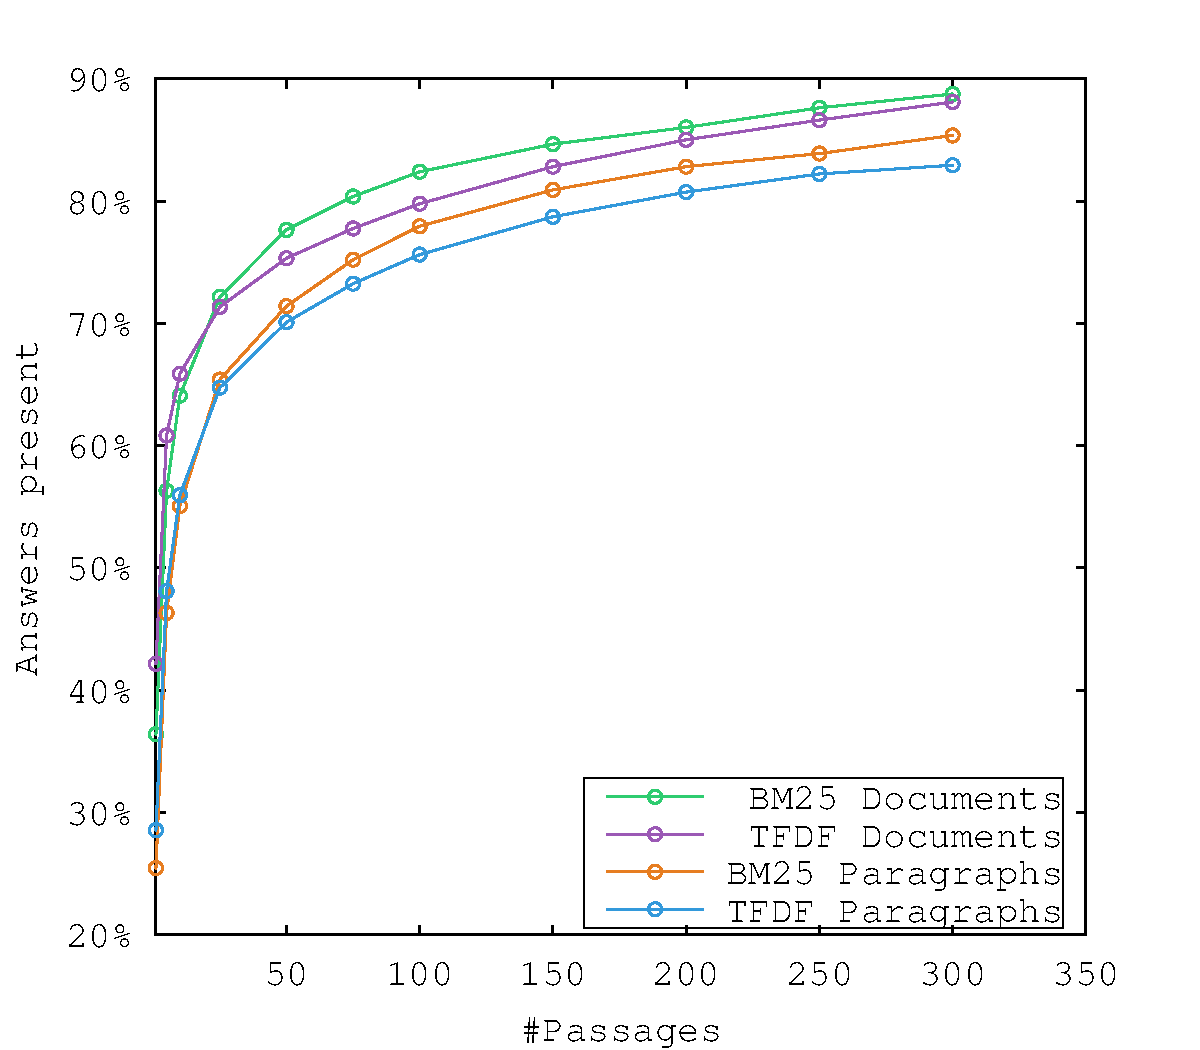
\includegraphics[width=0.5\textwidth]{figures/bm25_tfdf.pdf}
  \caption{Comparison between Lucene default, and BM25 similarities, when indexing by articles and paragraphs. 
  Shows how many percentages of the answers that were present for different number of passages.}
  \label{fig:bm25_tfdf}
\end{figure}

As we can see, BM25 is slightly better than Lucene default on all passages $>$ 25, and no result can be considered acceptable with passages $<$ 25.
Not surprisingly indexing by entire articles gives a better result than paragraphs, 
this can be explained by the fact that every article contains one or more paragraph. 
Which means that 100 article passages might yield the same amount of data as 200 paragraph passages.

\subsection{Noun extraction}


\begin{figure}[h!]
  \centering
  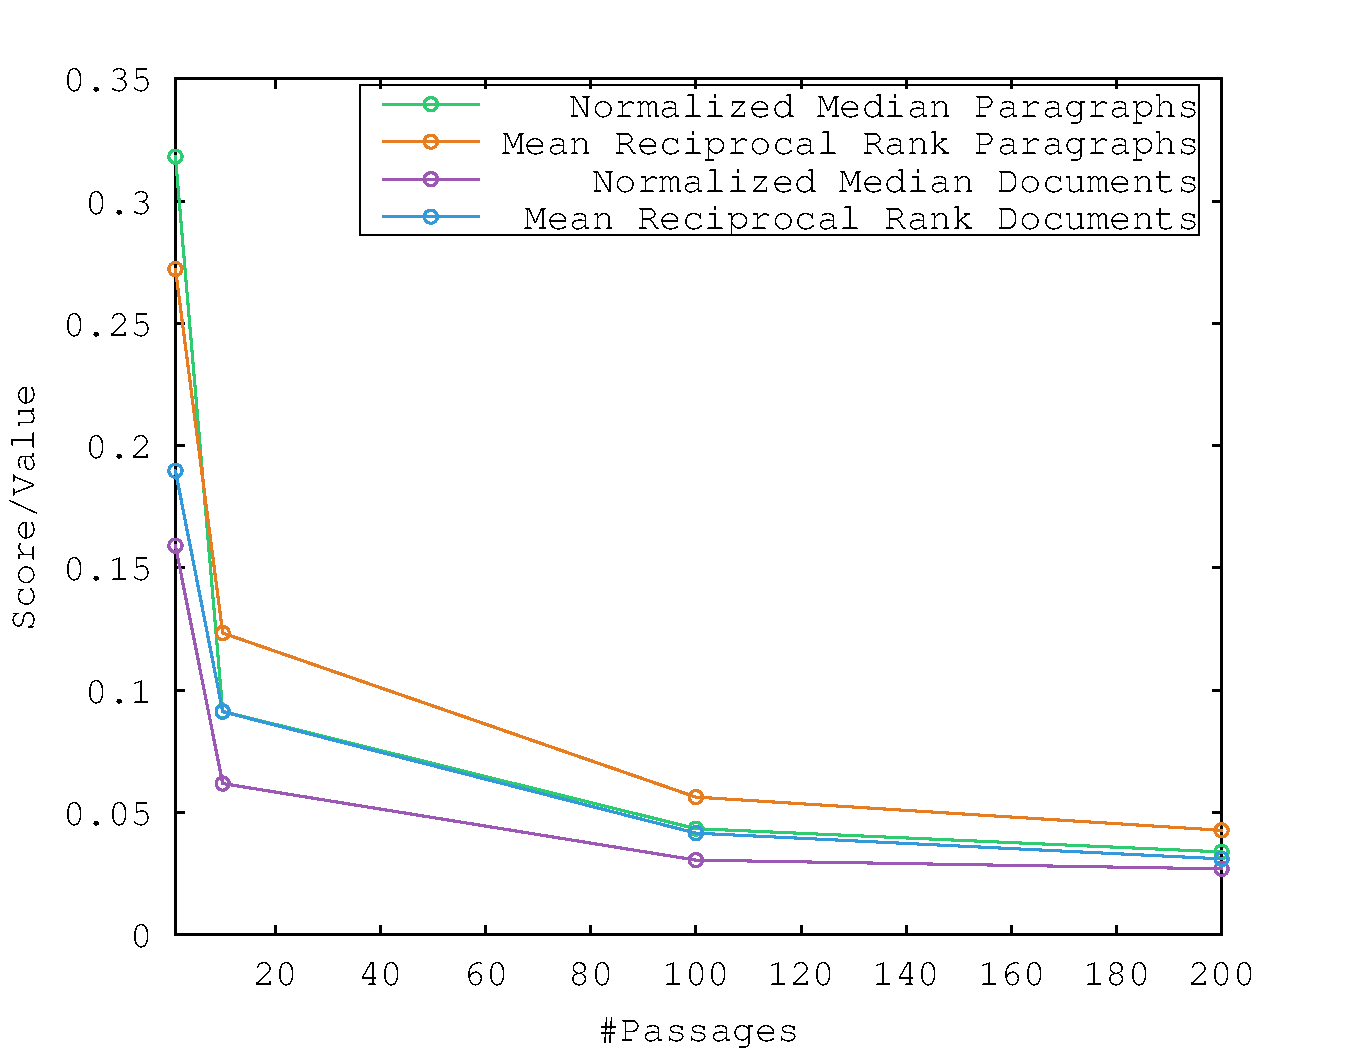
\includegraphics[width=0.5\textwidth]{figures/median.pdf}
  \caption{Comparison between indexing by articles, and indexing by paragraphs. 
  Shows the median and MRR values for the rank of the correct answer.}
\end{figure}

\subsection{Reranking}

\subsubsection{Median}


\begin{figure}[h!]
  \centering
  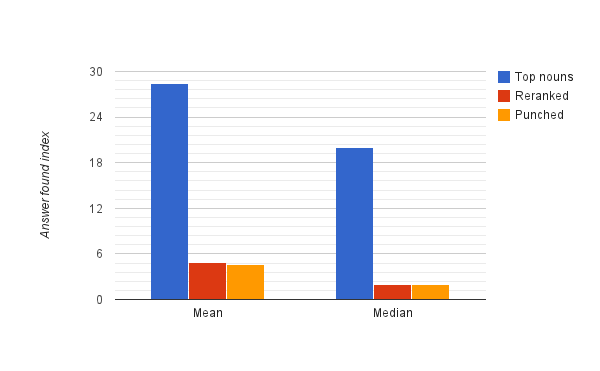
\includegraphics[width=0.5\textwidth]{figures/meanMedian.png}
  \caption{Comparison between indexing by articles, and indexing by paragraphs. 
  Shows the median and MRR values for the rank of the correct answer.}
\end{figure}

\subsubsection{MRR}


\begin{figure}[h!]
  \centering
  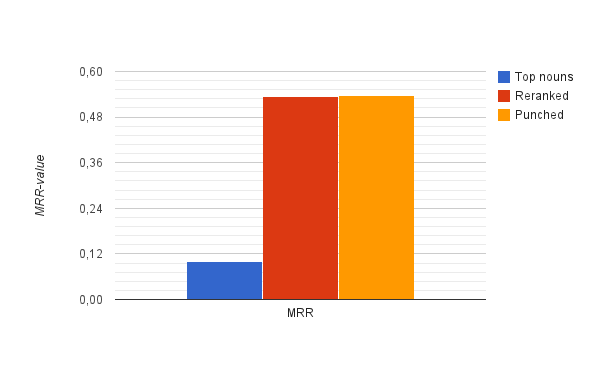
\includegraphics[width=0.5\textwidth]{figures/mrr.png}
  \caption{Comparison between indexing by articles, and indexing by paragraphs. 
  Shows the median and MRR values for the rank of the correct answer.}
\end{figure}
